%----------------------------------------------------------
\def\notedate{2021.11.14}
\def\currentauthor{Муха В. (РК6-73Б)}
%----------------------------------------------------------
\notestatement{rndhpcedt}{Известные алгоритмы поиска циклов в ориентированных графах}
%----------------------------------------------------------
%\subsubsection{}

Существует несколько групп алгоритмов поиска\cite{davidrajuh2016}:
\begin{enumerate}[label=\arabic*)]
    \item алгоритмы, основанные на обходе ориентированного графа (ОГ);
    \item алгоритмы, основанные на использовании матриц смежности, описывающих конкретный граф.
\end{enumerate}

Одним из представителей алгоритмов первой группы (обхода ОГ) является алгоритм поиска в глубину (англ., depth-first-search (DFS)), который предполагает, что обход осуществляется из фиксированного и заранее заданного узла. Если число узлов ОГ равно $n$, то сложность алгоритма DFS $O(n^2)$ и $O(n^3)$ -- для случая ``многократного обхода'' из каждого узла\footnote{Для случая ОГ возможность идентификации всех циклов требует осуществления многократных обходов, начиная с каждого из узлов ОГ.}. Поэтому для ускорения алгоритма необходимо применение модификаций, например распараллеливание алгоритма поиска в глубину~\cite{Mahdi2011}.

%Предполагая далее, что $n$ число узлов, з
Зададим граф $G(V, E)$, где $V = \{\bs{a}, \bs{b}, \bs{c}, \ldots\}$ -- множество вершин, $|V|=n$, а $E = \{\alpha\beta: \alpha\beta\in V\times V\}$ -- множество рёбер (пример, $\{\bs{ab}, \bs{ad}, \ldots , \bs{ge}\}$).

Для определения ОГ, часто, применяют понятие матриц смежности\cite{diestel2012graph}:
\begin{equation}\label{eq.rndhpcpar.2021.11.14.01}
\begin{array}{l}
||A||=||a_{ij}||_{n\times n};\\
a_{ij}=\left\{\begin{array}{l} 1, \mbox{ -- определено ребро с началом в узле $i$ и концом в узле $j$};\\ 0, \mbox{ -- ребро не определено}.\end{array} \right.
\end{array}
\end{equation}

\begin{equation}\label{eq.rndhpcedt.2021.11.14.00}
A=%
\begin{bmatrix}
	&	\bs{a}	&	\bs{b}	&	\bs{c}	&	\bs{d}	&	\bs{e}	&	\bs{f}	&	\bs{g} \\
\bs{a}	&	0	&	1	&	0	& 	1	& 	0	& 	0	 &	 0 \\
\bs{b}	&	0	&	0	&	0	& 	0	& 	1	& 	0	 &	 1 \\
\bs{c}	&	0	&	0	&	0	& 	0	& 	0	& 	1	 &	 0 \\
\bs{d}	&	1	&	0	&	1	& 	0	& 	0	& 	0	 &	 0 \\
\bs{e}	&	0	&	0	&	0	& 	0	& 	0	& 	1	 &	 0 \\
\bs{f}	&	0	&	0	&	1	& 	0	& 	0	& 	0	 &	 0 \\
\bs{g}	&	0	&	0	&	1	& 	1	& 	1	& 	01	 &	 0 \\
\end{bmatrix}
\end{equation}

Пример графа, построенного на основе его матрицы смежности $A$, приведен на рис.~\ref{fig.rndhpcpar.2021.11.14.01}.

%\begin{figure}[!ht]
%	\centering
%	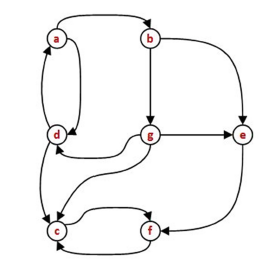
\includegraphics[width=0.3\textwidth]{ResearchNotes/rndhpc_not_par_2021_11_14/adj_matrix.png}
%	\caption{Граф, построенный по матрице смежности A}\label{fig.rndhpcpar.2021.11.14.01}
%\end{figure}

\begin{figure}[!ht]
	\centering
	\tikzstyle{circ} = [circle, text centered, draw=black]
	\tikzstyle{ar} = [->, >={Stealth[length=7pt]}]
	\tikzstyle{nt} = [text centered, color=black!50]
	\begin{tikzpicture}[align=center, auto]%, scale=1.16]
		\node[circ] (a) at (0,0) {$a$};
		\node[circ] (b) at (2,0) {$b$};
		\node[circ] (d) at (0,-2) {$d$};
		\node[circ] (g) at (2,-2) {$g$};
		\node[circ] (e) at (4,-2) {$e$};
		\node[circ] (c) at (0,-4) {$c$};
		\node[circ] (f) at (2,-4) {$f$};
		\draw [ar] (a) edge [bend left] (b);
		\draw [ar] (a) edge [bend left] (d);
		\draw [ar] (d) edge [bend left] (a);
		\draw [ar] (g) edge [bend left] (d);
		\draw [ar] (b) edge (g);
		\draw [ar] (g) edge (e);
		\draw [ar] (e) edge [bend left] (f);
		\draw [ar] (c) edge [bend left] (f);
		\draw [ar] (f) edge [bend left] (c);
		\draw [ar] (g) edge (c);
		\draw [ar] (d) edge [bend right] (c);
	\end{tikzpicture}
	\caption{Граф, построенный по матрице смежности A}\label{fig.rndhpcpar.2021.11.14.01}
\end{figure}

Элемент матрицы смежности $a_{ij}$ указывает на факт наличия определённого рёбра с началом в узле $i$ и концом в узле $j$, тогда как транспонированная матрица $A^T$ задаёт новый ОГ с теми же узлами и рёбрами, противоположно направленными относительно исходного ОГ.

\begin{equation}\label{eq.rndhpcpar.2021.11.14.02}
	A^T=%
	\begin{bmatrix}
		&	\bs{a}	&	\bs{b}	&	\bs{c}	&	\bs{d}	&	\bs{e}	&	\bs{f}	&	\bs{g} \\
	\bs{a}	&	0	&	0	&	0	& 	1	& 	0	& 	0	 & 	0 \\
	\bs{b}	&	1	&	0	&	0	& 	0	& 	0	& 	0	 & 	0 \\
	\bs{c}	&	0	&	0	&	0	& 	1	& 	0	& 	1	 & 	1 \\
	\bs{d}	&	1	&	0	&	0	& 	0	& 	0	& 	0	 & 	1 \\
	\bs{e}	&	0	&	1	&	0	& 	0	& 	0	& 	0	 & 	1 \\
	\bs{f}	&	0	&	0	&	1	& 	0	& 	1	& 	0	 & 	0 \\
	\bs{g}	&	0	&	1	&	0	& 	0	& 	0	& 	0	 & 	0 \\
	\end{bmatrix}
	\end{equation}

Введём обозначение матрицы, возведённой в степень $m$:
\begin{equation}\label{eq.rndhpcpar.2021.11.14.03}
A^m=\underbrace{A\times A \times \ldots \times A}_{m}.
\end{equation}

Матрица $A^m$ обладает следующим свойством: элемент матрицы $a^i_j$ равен числу путей из вершины $i$ в вершину $j$, состоящих ровно из $m$ рёбер\cite{diestel2012graph}. Длиной цикла называют количстево рёбер в этом цикле. Для того, чтобы определить циклы длины $2m$, нужно найти матрицу циклов $C_m$, определяемую следующим образом: 

\begin{equation}\label{eq.rndhpcpar.2021.11.14.04}
    C_m = A^m \wedge (A^T)^m;
\end{equation}
где $\wedge$ -- оператор конъюнкции, применяемый поэлементно.

Таким образом, матрица $C_m$ будет содержать все циклы длины $2m$. Пример для поиска циклов длины 2.~\ref{eq.rndhpcpar.2021.11.14.05}.
\begin{equation}\label{eq.rndhpcpar.2021.11.14.05}
	C_2 = A \wedge A^T = %
	\begin{bmatrix}
		&	\bs{a}	&	\bs{b}	&	\bs{c}	&	\bs{d}	&	\bs{e}	&	\bs{f}	&	\bs{g} \\
	\bs{a}	&	0	&	0	&	0	& 	1	& 	0	& 	0	 & 	0 \\
	\bs{b}	&	0	&	0	&	0	& 	0	& 	0	& 	0	 & 	0 \\
	\bs{c}	&	0	&	0	&	0	& 	0	& 	0	& 	1	 & 	0 \\
	\bs{d}	&	1	&	0	&	0	& 	0	& 	0	& 	0	 & 	0 \\
	\bs{e}	&	0	&	0	&	0	& 	0	& 	0	& 	0	 & 	0 \\
	\bs{f}	&	0	&	0	&	1	& 	0	& 	0	& 	0	 & 	0 \\
	\bs{g}	&	0	&	0	&	0	& 	0	& 	0	& 	0	 & 	0 \\
	\end{bmatrix}
	\end{equation}

%----------------------------------------------------------
% Атрибуты задачи
\noteattributes{}
%----------------------------------------------------------